\documentclass[11pt]{article}

\usepackage[margin=1in]{geometry}
\usepackage{amsmath}
\usepackage{graphicx}
\usepackage{hyperref}
\usepackage{booktabs}
\usepackage{array}

\hypersetup{
  colorlinks=true,
  linkcolor=blue,
  urlcolor=blue,
  citecolor=blue
}

\newcommand{\code}[1]{\texttt{#1}}
\newcommand{\DivB}{\nabla\cdot\mathbf{B}}
\newcommand{\Ndiv}{|\nabla\cdot\mathbf{B}|\Delta x/B_{\rm norm}}

% Auto-generated from the local AMR divB validation runs.
\newcommand{\StaticLevelRows}{%
1 & 9 & 3.203e-15 & 4.812e-17 & 6.278e-17 & 115200 \\%
2 & 9 & 3.576e-15 & 4.946e-17 & 6.493e-17 & 491520 \\%
3 & 9 & 3.546e-15 & 4.930e-17 & 6.483e-17 & 1839104 \\%
4 & 9 & 3.898e-15 & 5.037e-17 & 6.649e-17 & 6046720 \\%
5 & 9 & 3.641e-15 & 5.046e-17 & 6.663e-17 & 15784448 \\%
}
\newcommand{\TurbRows}{128}
\newcommand{\TurbPeakMaxNdiv}{7.597e-15}
\newcommand{\TurbPeakLoneNdiv}{1.158e-16}
\newcommand{\TurbPeakLtwoNdiv}{1.561e-16}
\newcommand{\TurbFinalMaxNdiv}{6.531e-15}
\newcommand{\TurbFinalLoneNdiv}{1.092e-16}
\newcommand{\TurbFinalLtwoNdiv}{1.469e-16}
\newcommand{\TurbMaxNcell}{2097152}
\newcommand{\TurbFinalNcell}{1713664}
\newcommand{\TurbTimeFinal}{1.600e-01}
\newcommand{\TurbCyclesFinal}{1261}
\newcommand{\FullGridNdivPfifty}{2.313e-17}
\newcommand{\FullGridNdivPninetyFive}{8.708e-17}
\newcommand{\FullGridNdivPninetyNine}{1.306e-16}
\newcommand{\FullGridNdivMax}{8.055e-16}


\title{Deep-AMR Face-Centered \texorpdfstring{$\nabla\cdot B$}{divB} Bug Fix Guide}
\author{AthenaK Gotham / MHD AMR validation notes}
\date{April 27, 2026}

\begin{document}
\maketitle

\section{Purpose}

This guide documents the face-centered MHD AMR bug that produced nonzero
\(\DivB\) in deep moving-AMR tests, what the code did before PR 732, what the
current code does, and how the current fix was validated.  The important point
is that the fix is not a divergence cleaner or projection.  It preserves the
constrained-transport AMR construction by making sure that the face fields used
by Toth--Roe prolongation and restriction are the correct face fields, owned by
the correct AMR path, at the correct time in the mesh rebuild.

\section{Discrete Constraint}

AthenaK MHD stores magnetic fields on faces.  For a cell \((i,j,k)\), the
finite-volume magnetic divergence is
\begin{equation}
  (\DivB)_{i,j,k} =
    \frac{B^1_{i+1/2,j,k} - B^1_{i-1/2,j,k}}{\Delta x_1}
  + \frac{B^2_{i,j+1/2,k} - B^2_{i,j-1/2,k}}{\Delta x_2}
  + \frac{B^3_{i,j,k+1/2} - B^3_{i,j,k-1/2}}{\Delta x_3}.
\end{equation}
On a uniform mesh, constrained transport preserves this to roundoff because the
same edge-centered electromotive forces update the two cells sharing a face.  On
AMR, this remains true only if coarse/fine face values are restricted,
prolongated, exchanged, and owned consistently.  If an active-domain face is
written twice, or if internal fine faces are computed from exterior faces that
later change, then the local discrete divergence constraint can be broken even
though the individual interpolation formulas are mathematically correct.

\section{Pre-PR 732 State}

Before the PR 732 boundary-ownership work, the face-centered AMR boundary path
had no sufficiently general active-face ownership rule.  A coarse-neighbor
\code{ProlongateFC} path could write faces that were already owned by a
same-level or finer neighbor at the same physical location.  This was most
visible around coarse/fine edges and corners, where a single prolongation buffer
range can include a mixture of true ghost faces and active-domain faces.  In 1D
this is hard to expose; in 2D and 3D, repeated moving refinement patterns expose
it quickly.

The original bug was therefore not ``MPI-IO-like nondeterminism'' or a failure
of CT itself.  It was an AMR ownership bug: different boundary paths disagreed
about which path owned the final value of a face-centered magnetic field.

The archival pre-732 comparison in Fig.~\ref{fig:pre732_current} shows the size
of the error on the original moving-AMR diagnostic.  The 2D and 3D failures were
at the \(10^{-3}\) level in normalized maximum divergence, while the current
code is at roundoff.  The plotted current 3D value uses the common two-physical
AMR-level depth so that the comparison is against the same style of test that
originally exposed the bug.

\begin{figure}[htbp]
  \centering
  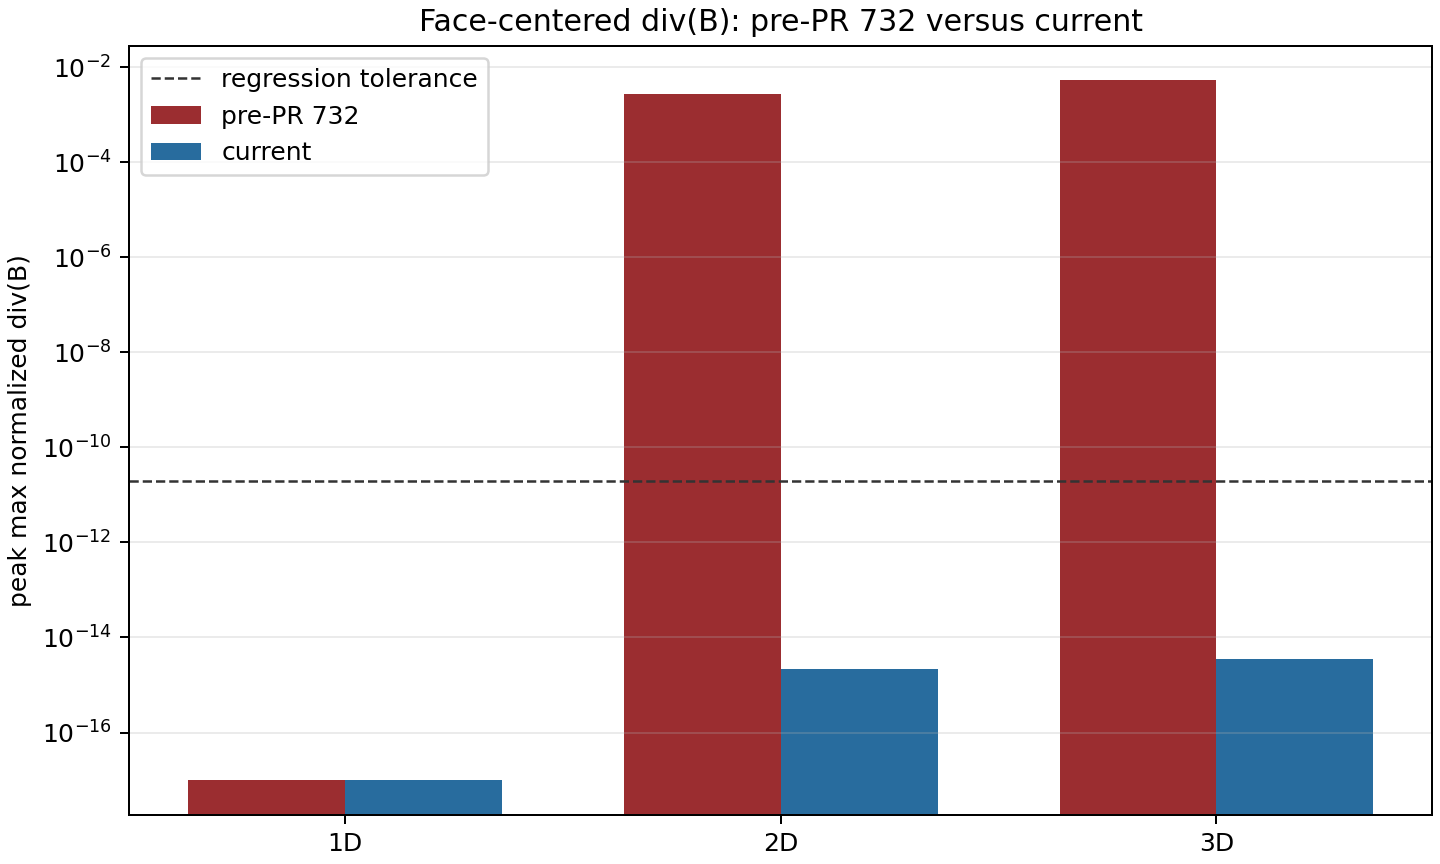
\includegraphics[width=0.78\linewidth]{figures/divb_amr_pre732_vs_current.png}
  \caption{Archival pre-PR 732 moving-AMR result compared with the current code.
  The current result is many orders of magnitude below the regression tolerance.}
  \label{fig:pre732_current}
\end{figure}

\section{Why PR 732 Was Necessary But Not Sufficient}

PR 732 fixed an important part of the problem: coarse-neighbor boundary
prolongation should not overwrite faces owned by same-level or finer neighbors.
That change was necessary.  However, deeper 3D tests still failed.  The failure
pattern was the clue: one or two physical AMR levels were clean, while three or
more levels produced large \(\DivB\) after rebuilds.  That behavior pointed away
from a simple analytic prolongation error and toward an ordering/ownership error
that only appears when refinement and derefinement interact across multiple
levels.

The critical remaining issue was stale restricted face data during
derefinement.  In the mesh-rebuild routine, AMR send buffers are prepared before
same-rank derefine copies are performed.  Before the current fix, the MHD
derefine path could pack or copy \code{coarse\_b0} that had not been freshly
restricted from the current \code{b0}.  With shallow AMR this often escapes
detection.  With deep AMR, stale coarse magnetic faces can seed a new block or a
neighbor boundary with a value that is not the restriction of the current fine
state.  Subsequent CT-consistent operations then preserve the wrong local face
balance.

\section{Current Code State}

The current implementation has four coordinated pieces.

\subsection{Refresh Coarse Face Fields Before AMR Packing}

After the final \code{refine\_flag} values are known and synchronized, but before
\code{InitRecvAMR()} and \code{PackAndSendAMR()}, the code now refreshes the MHD
coarse face-centered storage when derefinement is present:
\begin{verbatim}
if ((ndel > 0) && (pmhd != nullptr)) {
  RestrictFC(pmhd->b0, pmhd->coarse_b0);
}
\end{verbatim}
This is the most important correctness fix for the deep-AMR failures.  It makes
the derefine send/copy source data match the current fine face-centered fields.

\subsection{Exact Active-Face Ownership During Boundary Prolongation}

\code{src/bvals/prolongation.cpp} now routes face-centered boundary
prolongation writes through \code{CanProlongateFCFace()} and
\code{StoreProlongatedFCFace()}.  The predicate allows ghost-face writes, but it
allows active-domain writes only when the face is the normal interface face
owned by the coarse-neighbor prolongation path and no same-level or finer
neighbor owns that face.  Active interior faces are not written by the boundary
prolongation path.

This replaces broad range clipping with an exact per-face decision.  That
matters at edges and corners because a rectangular buffer range can contain both
faces that the coarse neighbor should supply and faces that must be left to a
same-level/finer neighbor or to the local active state.

\subsection{Protect Active Faces During Same/Finer Receives}

\code{MeshBoundaryValuesFC::RecvAndUnpackFC()} now skips same-level and finer
receive-buffer writes that target active-domain faces.  Direct receive unpacking
is still used for ghost data, but it no longer overwrites active magnetic faces
through overlapping edge/corner communication paths.

Debug prints for blocked writes are available behind
\code{ATHENAK\_DEBUG\_FC\_AMR\_OWNERSHIP}.  Production builds pay no always-on
provenance cost.

\subsection{Post-Boundary AMR Face Repair}

\code{RepairAMRFC()} is called after boundary values and primitives are
initialized.  It recomputes internal face-centered fields for AMR-affected
MeshBlocks after exterior faces have been finalized by boundary exchange and
prolongation.  In multidimensions it reuses the same Toth--Roe internal-face
prolongation operator; in 1D it keeps the existing midpoint face average.  It
does not alter exterior block faces.

The repair mask is broader than ``newly refined only.''  It marks blocks whose
own old source changed level and local blocks adjacent to level-changed
neighbors.  This is deliberately conservative: the extra work happens only
immediately after AMR topology changes, and the affected blocks are precisely
where exterior face values may have changed during the rebuild.

After repair, MHD primitives are recomputed from the repaired face fields.  This
keeps total energy, magnetic pressure, and characteristic speeds consistent with
the final magnetic state.  No divergence cleaning, projection, or user input
control is introduced.

\section{Regression and Stress Tests}

The validation uses a \code{divb\_amr} problem generator that initializes the
field from a discrete vector potential, so the initial face-centered field is
divergence-free to roundoff.  The refinement pattern is intentionally artificial
and moving.  It is designed to repeatedly create coarse/fine faces, edges, and
corners rather than to follow a passive physical threshold.

The strict pass criteria are
\begin{align}
  \max(\Ndiv) &< 2\times10^{-11},\\
  L_1(\Ndiv) &< 2\times10^{-12},\\
  L_2(\Ndiv) &< 5\times10^{-12}.
\end{align}

\subsection{Static Moving-AMR Level Sweep}

The deterministic 3D moving-AMR sweep now tests one through five physical AMR
levels.  The current code passes all depths at roundoff.  This is the primary
gate because the earlier one- or two-level tests were not discerning enough.

\begin{table}[htbp]
  \centering
  \caption{Current 3D static moving-AMR level sweep, run with 8 MPI ranks.}
  \small
  \begin{tabular}{@{}rrrrrr@{}}
    \toprule
    Levels & Rows & Peak max & Peak \(L_1\) & Peak \(L_2\) & Max cells\\
    \midrule
    \StaticLevelRows
    \bottomrule
  \end{tabular}
  \label{tab:static_sweep}
\end{table}

\begin{figure}[htbp]
  \centering
  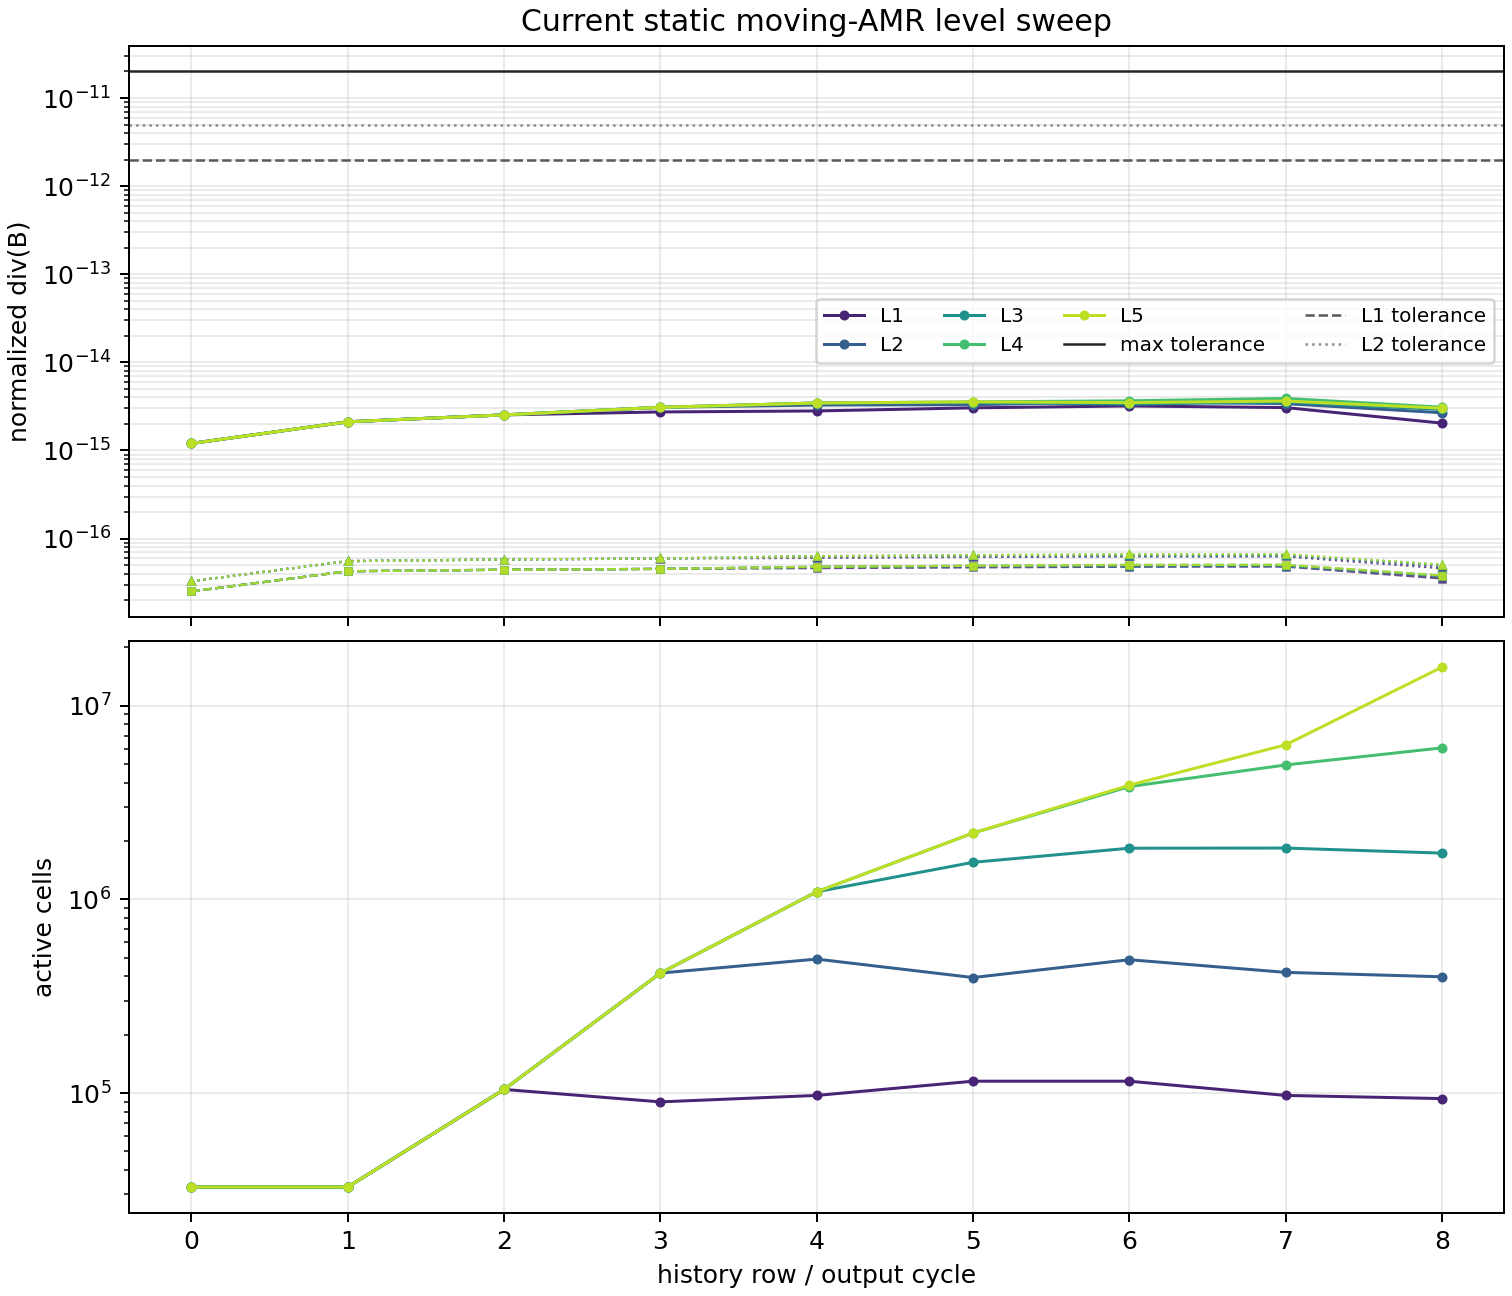
\includegraphics[width=0.86\linewidth]{figures/divb_amr_static_level_sweep_current.png}
  \caption{Current static moving-AMR level sweep.  All depths remain many orders of
  magnitude below the strict normalized-divergence tolerances.}
  \label{fig:static_sweep}
\end{figure}

\subsection{Driven Turbulence Stress Test}

The driven case uses the same 3D AMR diagnostic with MHD turbulent driving:
\begin{itemize}
  \item \(32^3\) root grid with \(8^3\) MeshBlocks;
  \item three physical refinement levels, giving an effective finest resolution of
    \(256^3\);
  \item periodic boundaries, ideal MHD, PLM reconstruction, HLLD;
  \item \code{dedt = 75}, \code{tcorr = 0.002}, \code{nlow = 1},
    \code{nhigh = 3};
  \item completed retained-output run to \(t=\TurbTimeFinal\).
\end{itemize}

The retained binary figures are from a completed short diagnostic run.  That run
wrote history every cycle, binary slices every 0.001 code time, and full-cube
binary diagnostics every 0.002 code time.  It was executed with 8 MPI ranks
using the current repaired code.  This run is useful as a driven-AMR stress
check, but it should not be described as a two-eddy-turnover turbulence run.

A corrected longer diagnostic input under \code{inputs/tests} now targets
\(t=0.16\), roughly two forcing-scale eddy turnover times for a Mach
\(\sim0.5\) state in this unit box.  That input writes slices every 0.02 code
time and full-cube diagnostics every 0.08 code time.  On the local laptop the
attempted long run caused memory pressure and was stopped before completion, so
the final long-run slice files were not retained.  The partial history that was
visible before cleanup reached \(t\simeq\PartialLongTurbTime\) with peak
\(\max(\Ndiv)\simeq\PartialLongTurbPeakMaxNdiv\), peak
\(L_1\simeq\PartialLongTurbPeakLoneNdiv\), and peak
\(L_2\simeq\PartialLongTurbPeakLtwoNdiv\).  This partial result is encouraging
but is not a substitute for a completed two-eddy-turnover run on a machine with
enough memory.

The peak normalized divergences over the retained completed driven run were
\begin{align}
  \max(\Ndiv) &= \TurbPeakMaxNdiv,\\
  L_1(\Ndiv) &= \TurbPeakLoneNdiv,\\
  L_2(\Ndiv) &= \TurbPeakLtwoNdiv.
\end{align}
The final retained-output values were
\begin{align}
  \max(\Ndiv) &= \TurbFinalMaxNdiv,\\
  L_1(\Ndiv) &= \TurbFinalLoneNdiv,\\
  L_2(\Ndiv) &= \TurbFinalLtwoNdiv.
\end{align}
The maximum active-cell count was \(\TurbMaxNcell\), and the final active-cell
count was \(\TurbFinalNcell\).

\begin{figure}[htbp]
  \centering
  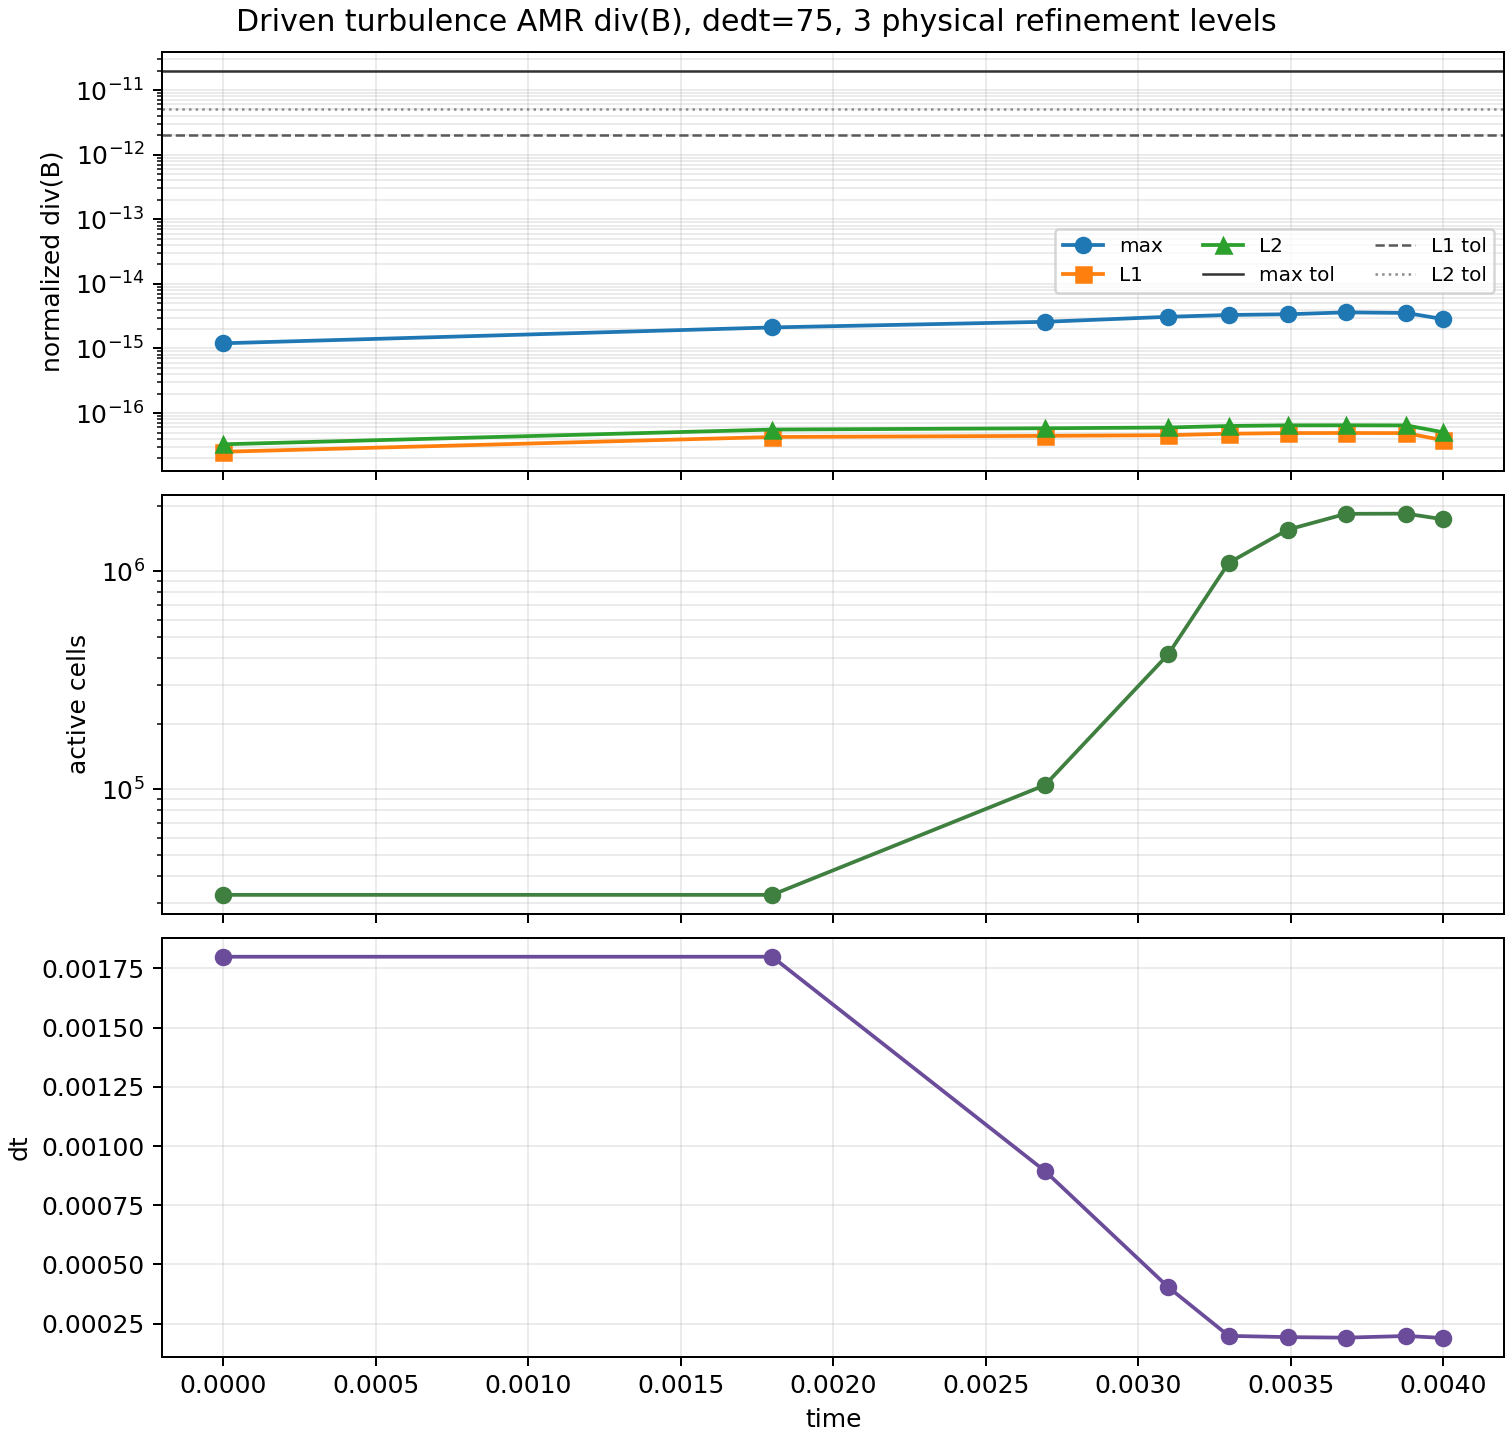
\includegraphics[width=0.86\linewidth]{figures/divb_amr_turb_edot75_l3_history.png}
  \caption{Retained driven turbulence AMR history for \code{dedt = 75} and three
  physical refinement levels.  The AMR hierarchy changes aggressively and the
  divergence diagnostics remain at roundoff, but this retained run stops at
  \(t=0.004\), not at two eddy turnover times.}
  \label{fig:turb_history}
\end{figure}

The retained final full-cube visualization distribution is also clean.  On the
uniformized retained final binary cube, the 50th, 95th, and 99th percentiles of
\(\Ndiv\) are \(\FullGridNdivPfifty\), \(\FullGridNdivPninetyFive\), and
\(\FullGridNdivPninetyNine\).  The maximum in the uniformized visualization cube
is \(\FullGridNdivMax\).  The history file remains the authoritative
finite-volume diagnostic because it is accumulated directly over the AMR mesh.

\begin{figure}[htbp]
  \centering
  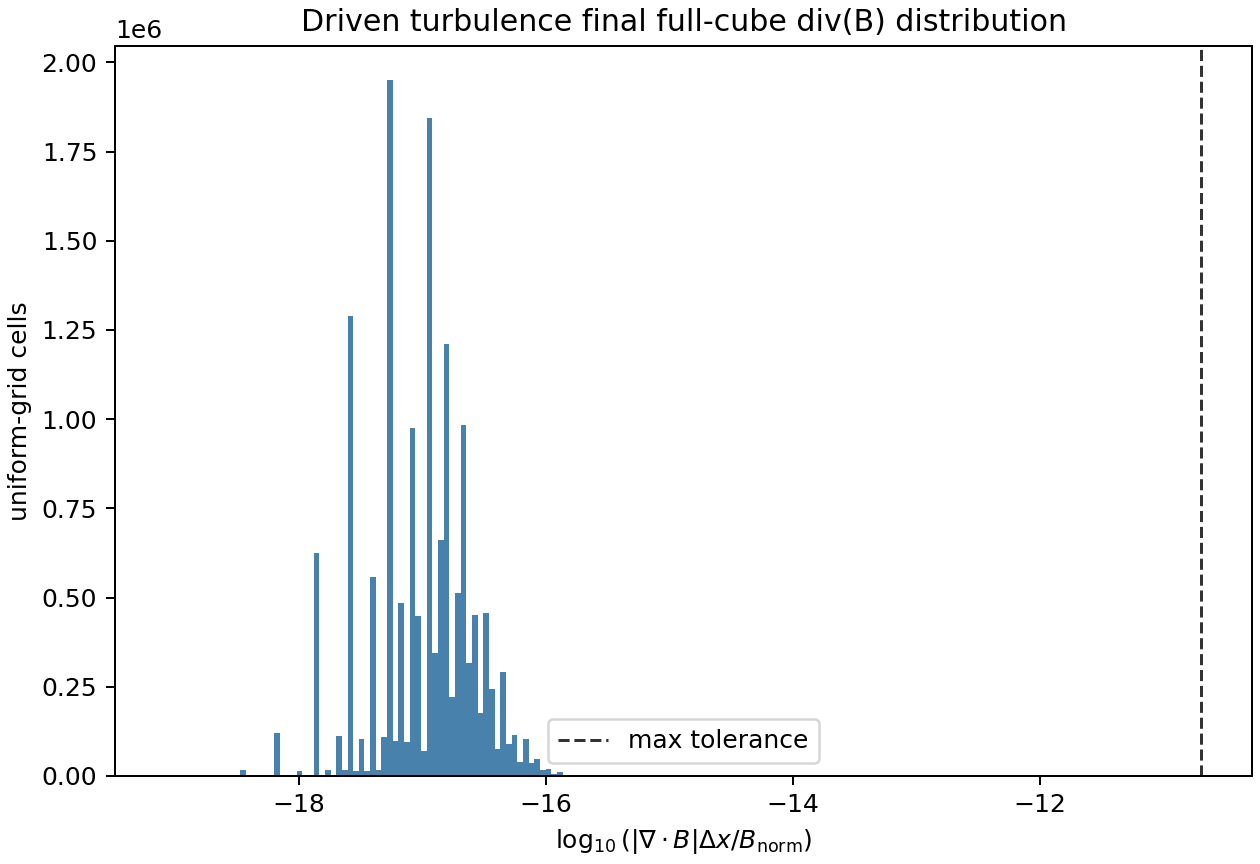
\includegraphics[width=0.74\linewidth]{figures/divb_amr_turb_edot75_l3_divb_distribution.png}
  \caption{Retained short-run full-cube normalized-divergence distribution from
  the driven turbulence diagnostic output.}
  \label{fig:turb_distribution}
\end{figure}

\begin{figure}[htbp]
  \centering
  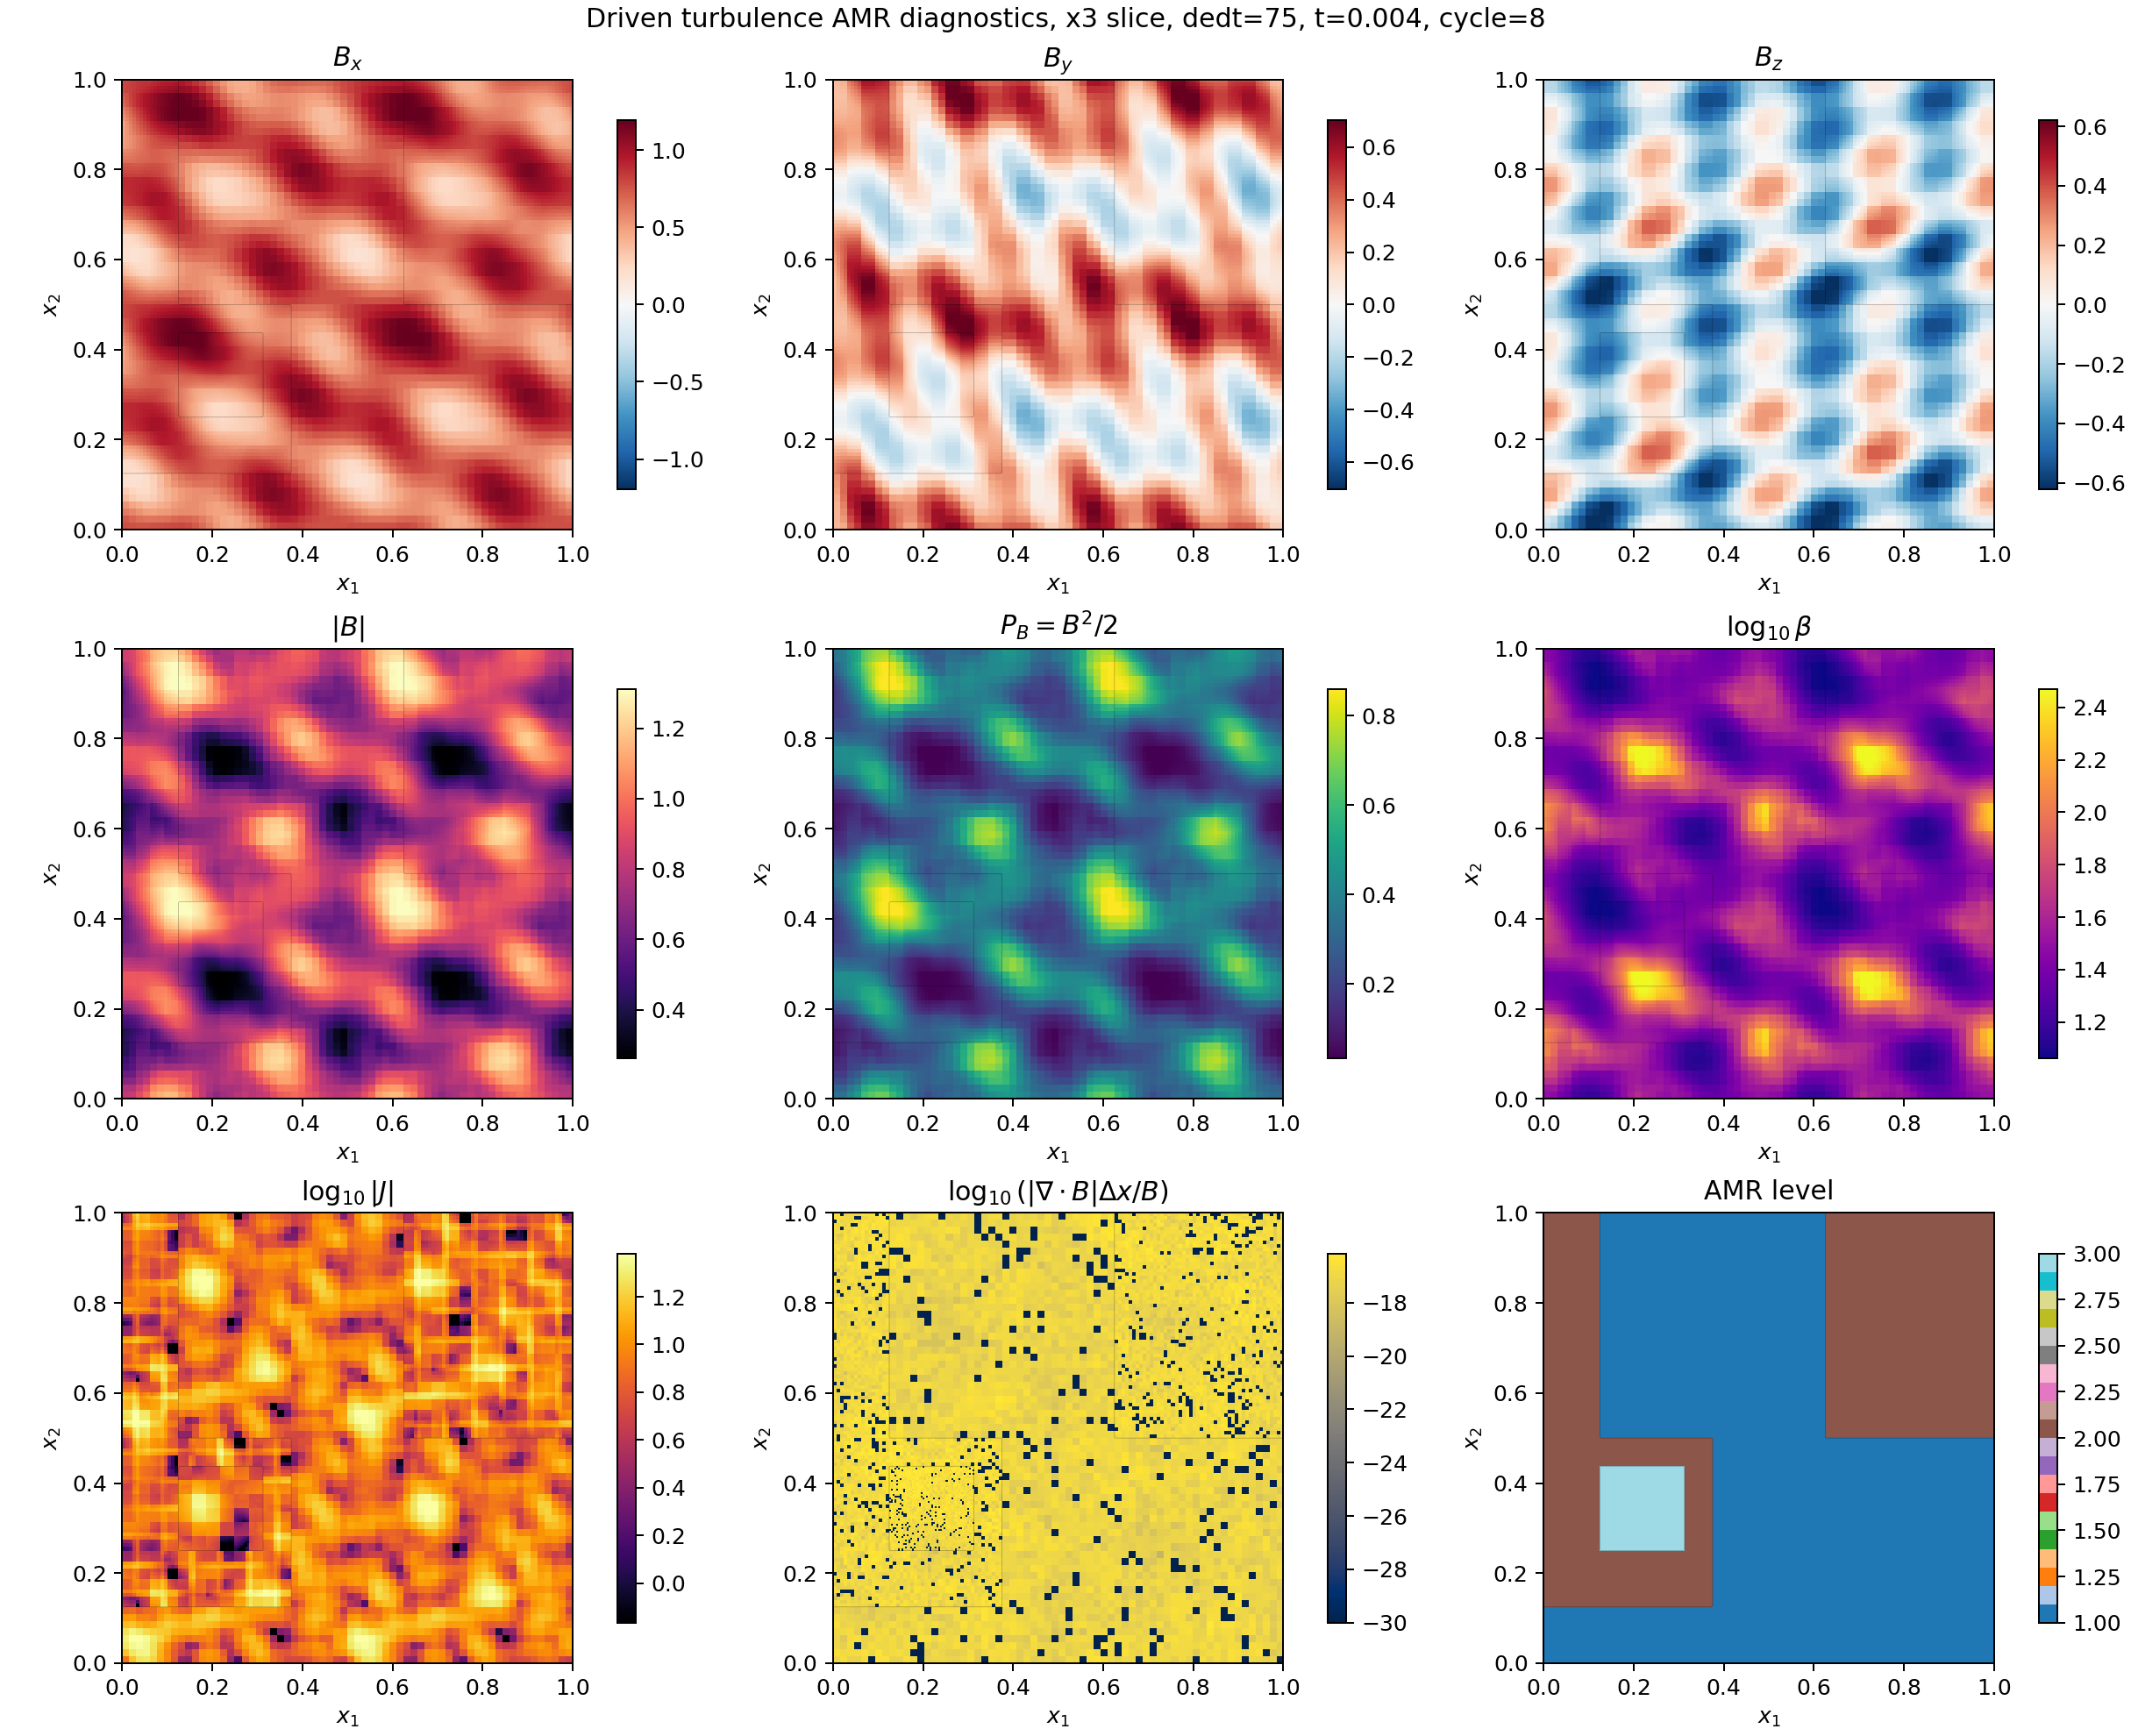
\includegraphics[width=0.98\linewidth]{figures/divb_amr_turb_edot75_l3_x3_slice.png}
  \caption{Retained short-run \(x_3=0.5\) slice diagnostics from the driven
  turbulence test. Magnetic-field structure, current density, and AMR level
  boundaries are visible, while normalized \(\DivB\) remains at roundoff.}
  \label{fig:turb_x3}
\end{figure}

\begin{figure}[htbp]
  \centering
  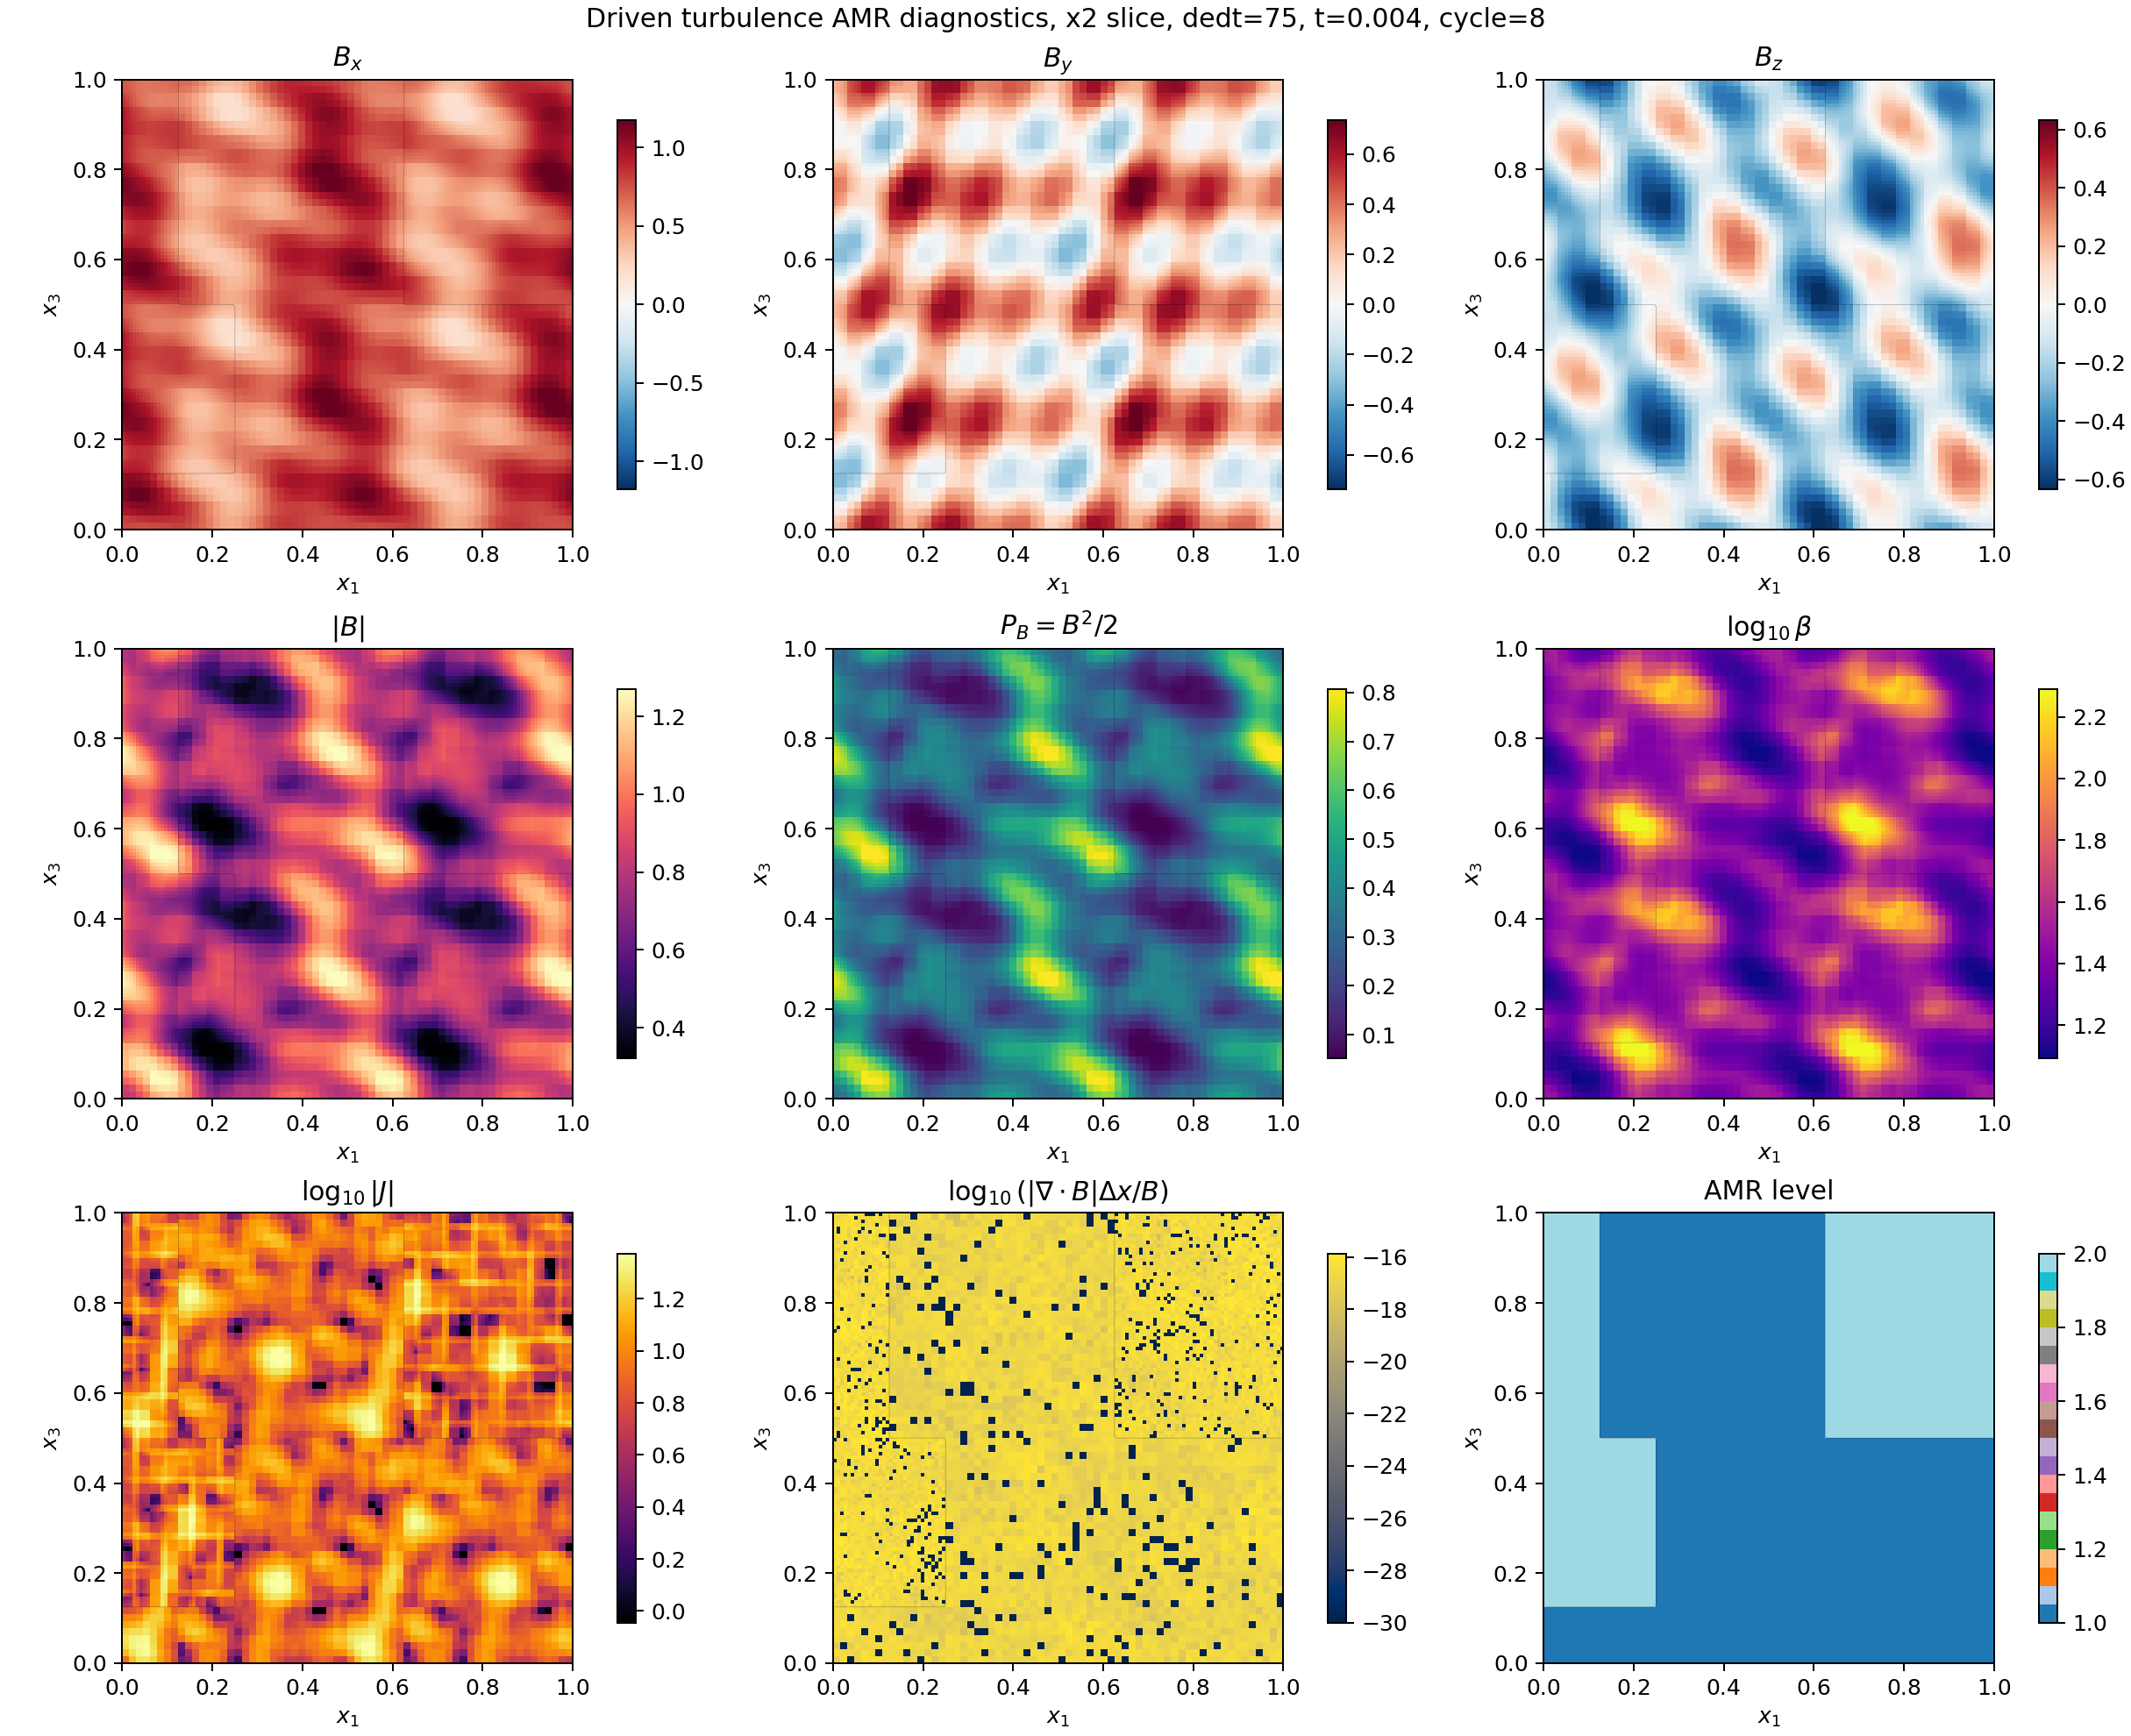
\includegraphics[width=0.98\linewidth]{figures/divb_amr_turb_edot75_l3_x2_slice.png}
  \caption{Retained short-run \(x_2=0.5\) slice diagnostics from the same driven
  turbulence test.}
  \label{fig:turb_x2}
\end{figure}

\section{Runtime and Speed}

The current fixes are deliberately scoped to AMR and boundary work:
\begin{itemize}
  \item \code{RestrictFC()} is called before AMR packing only when derefinement
    occurs and MHD is active.
  \item The exact face-ownership predicate is evaluated only in face-centered
    boundary prolongation and only on the coarse-neighbor path.
  \item \code{RepairAMRFC()} runs only after AMR topology changes and only on
    blocks marked by the AMR repair mask.
  \item \code{ATHENAK\_DEBUG\_FC\_AMR\_OWNERSHIP} diagnostics are off unless the
    code is built with that macro.
\end{itemize}

The retained short \code{dedt = 75} diagnostic run completed in 21.72 seconds of
wall time on the local 8-rank test.  AthenaK reported 16157 MeshBlock-cycles,
10.18 seconds of CPU time, and \(8.12\times10^5\) zone-cycles per CPU-second.
For comparison, the static 3-level run with the same MeshBlock-cycle count
reported 7.54 CPU seconds and \(1.10\times10^6\) zone-cycles per CPU-second.
The driven run is expected to be slower because it includes turbulent driving
and extra full-cube/slice diagnostic outputs.  The post-setup diagnostic-output
time in the retained short run was only 0.099 seconds total, with 0.050 seconds
spent in writes.  The attempted longer laptop run was memory-limited rather than
diagnostically complete, so no speed conclusion should be drawn from that
interrupted attempt.

I did not run a same-physics pre-fix versus post-fix performance A/B benchmark
in this pass, because the pre-fix code fails the correctness test at three or
more physical AMR levels.  From the code path and the local timings, the new
correctness work does not appear to be a dominant runtime cost.  If exact
overhead matters for production performance estimates, the right follow-up is a
two-binary benchmark with the same problem, same AMR rebuild schedule, and the
debug macro disabled in both builds.

\section{Practical Checklist for Future Changes}

Future MHD AMR changes should preserve the following invariants:
\begin{enumerate}
  \item A face-centered active-domain face has one owner during an AMR rebuild.
  \item Same-level and finer receive/prolongation paths may fill ghost data but
    must not overwrite active faces.
  \item Coarse-face storage used for derefinement must be freshly restricted
    before AMR send buffers are packed.
  \item Toth--Roe internal fine faces must be computed after exterior faces have
    their final AMR-boundary values.
  \item Primitive recovery must run after any face-centered repair that can
    change magnetic energy or characteristic speeds.
\end{enumerate}

The current deterministic regression should keep the 3D physical level sweep
through at least five levels.  One or two physical levels are not a sufficient
proof of correctness for this bug class.

\end{document}
